\documentclass[UTF8,noindent]{ctexart}
\usepackage[a4paper,left=2.0cm,right=2.0cm,top=2.0cm,bottom=2.0cm]{geometry}
\usepackage{graphicx}
\usepackage{amsmath}
\usepackage{amssymb}
\usepackage{xeCJK}
\usepackage{listings}
\usepackage{float}
\CTEXsetup[format={\Large\bfseries}]{section}

\title{$Project1-Bootloader$ 设计文档}

\author{冯吕$\quad 2015K8009929049$}
\date{\today}
\begin{document}
\maketitle
\zihao{5}
\CJKfamily{zhsong}

\section*{一、$Task2$:输出字符串}

$PMON $下的字符输出为串口输出,地址为$ 0xbfe48000$,因此,要输出字符,只需不停向该地址写字符即可。

实现的代码如下:
\begin{lstlisting}
  .data
        str: .asciiz "Welcome to OS!\n"
  .text
       .globl main

  main:
# check the offset of main
	nop
	nop
	nop
	nop
	nop
	nop
	nop
	nop
	nop
	nop
	nop
	nop

	la $8, str
	li $10, 0xbfe48000

putstr:
	lb $9, ($8)
	beq $9, $0, end
	sb $9, ($10)
	addiu $8, 1
	j putstr
end:
	nop
\end{lstlisting}

首先声明一个字符串$str$,然后将其地址加载到$8$号寄存器,取出一个字符,判断是否为$0$,如果不是,则输出,
然后地址加一,返回继续输出,如果是,则结束。

该任务主要在于循环的实现,以及$lb$和$sb$指令的使用,不可以使用$lw$和$sw$指令,因为串口输出是字符输出,
如果使用$lw$和$sw$指令则会导致出错。\\

输出截图:
\begin{figure}[H]
	\centering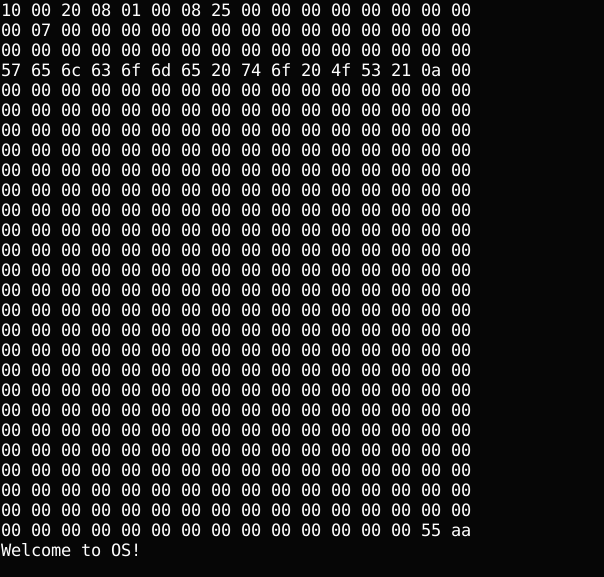
\includegraphics[height = 9cm, width = 
	13cm]{fig/2.png}\caption{串口字符串输出}
\end{figure}

\section*{二、$Task3: Bootloader$开发}
需要实现的$bootblock$的功能是首先将内核从启动设备($U$盘)加载到内存中,然后跳转到内核中$main$函数的
起始处开始执行。

$PMON$中读盘函数的地址为$0x8007b1a8$,在调用该读盘函数时,需要向其传递三个参数:
\begin{itemize}
	\item 第一个参数为读取的目的地址,即读取的数据在内存存放的位置;
	\item 第二个参数为SD卡内部的偏移量,从该处开始读取;
	\item 	第三个参数为要读取的字节数。
\end{itemize}

在$MIPS$汇编中,函数调用的参数传递是通过$4,5,6,7$号寄存器传递的,若参数超过$4$个,则多余参数通过栈传递。
因此,这里只需要使用$4,5,6$号寄存器即可。

在调用读盘函数的时候,首先,将三个参数加载到寄存器中,然后使用$JAL$指令跳转到读盘函数所在的地址,
从而完成函数调用,将内核加载到内存中。之后再跳转到内核中$main$函数所在的地方开始执行。

实现的代码如下:
\begin{lstlisting}
	.text
	.globl main

main:
# check the offset of main
	nop
	nop
	nop
	nop
	nop
	nop
	nop
	nop
	nop
	nop
	nop
	nop

	li $4, 0xa0800200
	li $5, 0x200
	li $6, 0x200
	jal 0x8007b1a8
	jal 0xa080026c
\end{lstlisting}

实际上,加载完内核以后,跳转到内核中$main$函数的开始处执行其实也就是调用$main$函数,因此,仍然需要使用
$JAL$指令。\\

开发过程中遇到的问题以及解决办法:
\begin{enumerate}
	\item 如何确定读盘函数的三个参数:对于内核加载到内存中的地址,需要通过读取内核文件来获取,即
	程序段所对应的虚拟地址:$0xa0800200$;对于内核在启动盘中的偏移和需要读取的字节数,由于$bootblock$
	和$kernel$在镜像中各占一个扇区,一个扇区的大小为$512$个字节,因此,偏移量和需要读取的字节数均为
	$0x200$。从而,确定了读盘函数的三个参数。
	\item 
	刚开始开发的时候,使用$J$指令跳转到内核中$main$函数的开始处执行指令,导致不停输出\emph{It's
	 kernel!}。发生该错误的原因是,在$MIPS$汇编中,函数调用会把返回地址保存在$31$号寄存器,在上一条
 调用读盘函数的指令中,将返回地址保存到了$31$号寄存器,而此时使用$J$指令不是函数调用,因此$31$号寄存器的
 内容没有更新,还保存着之前的返回地址。所以从$main$函数返回后又回到了相同的地方,导致不停调用$main$函数,
 于是不停输出\emph{It's 
 kernel!}。解决办法:只需将$J$指令改为$JAL$指令即可,使用$JAL$指令,则$31$号寄存器的内容会更新为调用
 $main$函数这条指令所在的地址,因此,函数返回以后往后面执行,不会继续调用$main$函数。
\end{enumerate}

输出截图:
\begin{figure}[H]
	\centering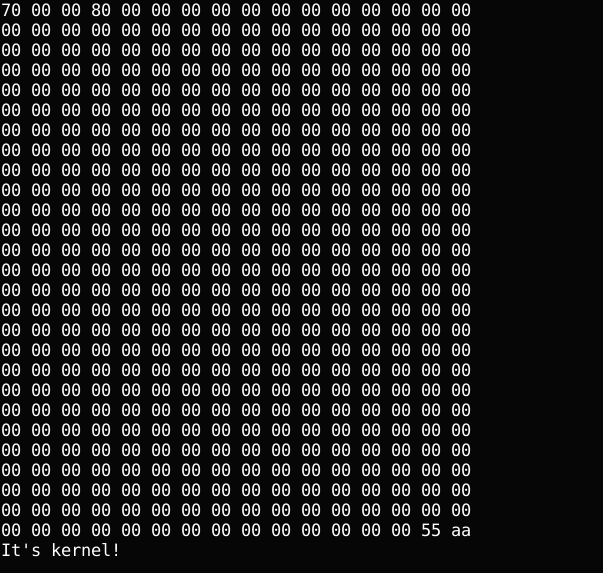
\includegraphics[height = 9cm, width = 
	13cm]{fig/3.png}\caption{串口输出\emph{It's kernel!}}
\end{figure}

\section*{三、$createimage$开发}
该任务是开发一个$Linux$工具,利用$bootblock$和$kernel$编译后的二进制文件创建一个启动镜像。实际就是将
$bootblock$二进制文件中的可加载程序段和$kernel$二进制文件中的可加载程序段合并写为一个镜像文件,其
中$bootblock$位于镜像文件的第一个扇区,$kernel$位于第二个扇区。由于程序段的长度小于一个扇区,因此不
满的一个扇区的地方置为$0$。

要获取$bootblock$和$kernel$二进制文件中的可执行程序段,首先需要读取$ELF$文件头表,从而知道程序头表
在文件中的偏移。知道程序头表在文件中的偏移以后,便可读出程序头表。之后,根据文件头表和程序头表,便可知道
几乎关于文件的一切信息了,从而找出可执行程序段,写入镜像中。\\

读取二进制文件中可执行代码创建镜像的过程:

使用$fread()$函数读取$ELF$文件头表到$ehdr$所指向的缓冲区$\longrightarrow$使用$fseek()$函数将文件指针
指到第$ehdr->e\_phoff$处(即为程序头表开始处)$\longrightarrow$再次使用$fread()$函数将程序头表
读取到$phdr$所指向的内存缓冲区中$\longrightarrow$对于每一个程序段,判断$phdr->p\_type$是否等于
$PT\_LOAD$,即是否是可加载的$\longrightarrow$若是,利用$fseek()$函数将文件指针指到文件的第
$phdr->p\_offset$个字节处($phdr->p\_offset$即为程序段在文件中的偏移)$\longrightarrow$从该处
读取$phdr->p\_filesz$个字节到内存中$\longrightarrow$再将其写入镜像文件中。

以上即为读取文件创建镜像的基本过程。\\

为了让$bootblock$知道$kernel$的大小,即向读盘函数传递第三个参数,我的实现方法是直接在$createimage$
中计算出$kernel$的大小,然后通过修改$image$文件来传递参数。\\

开发过程中遇到的问题:
\begin{enumerate}
	\item 如何读取$ELF$文件:刚开始,不了解$ELF$文件格式,因此无从下手,后来通过查阅相关材料,
	了解了$ELF$文件,然后才知道该如何读取;
	\item 镜像文件写入错误:刚开始,读取文件正确,但写出的镜像文件不正确,后来发现原因是,我直接将程序段
	从一个文件流写入另一个文件流,这样做错误的,而应该先读入内存,然后再写进镜像文件;
	\item 如何计算$bootblock$和$kernel$的长度:利用文件头表和程序头表无法计算出长度,
	而需要使用$sys/stat.h$头文件中的$stat()$函数才能够获取长度。
	\item 
	如何在$createimage$中向$bootblock$传参:直接修改镜像文件中的指令来传参。将$bootblock.s$中
	传递第三个参数的指令写为$nop$指令,然后在$createimage$中将此指令更改为传参指令。
\end{enumerate}

编译截图:
\begin{figure}[H]
	\centering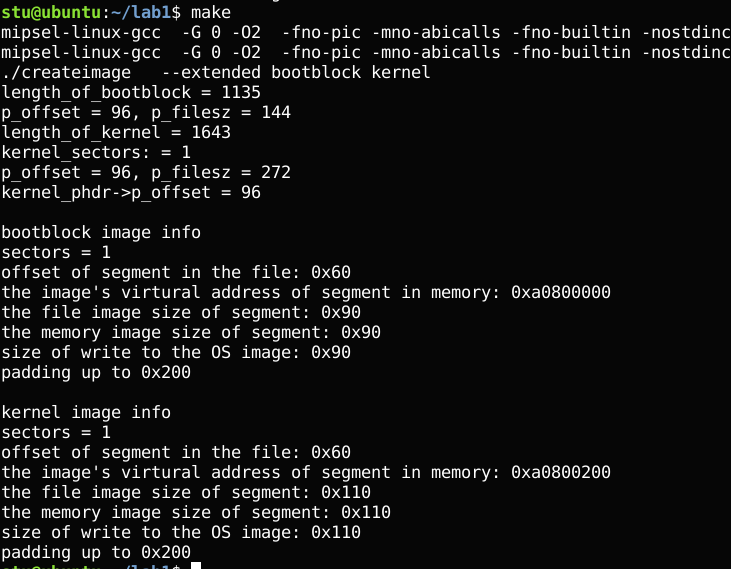
\includegraphics[height = 9cm, width = 
	13cm]{fig/4.1.png}\caption{输出镜像相关信息}
\end{figure}

输出截图:
\begin{figure}[H]
	\centering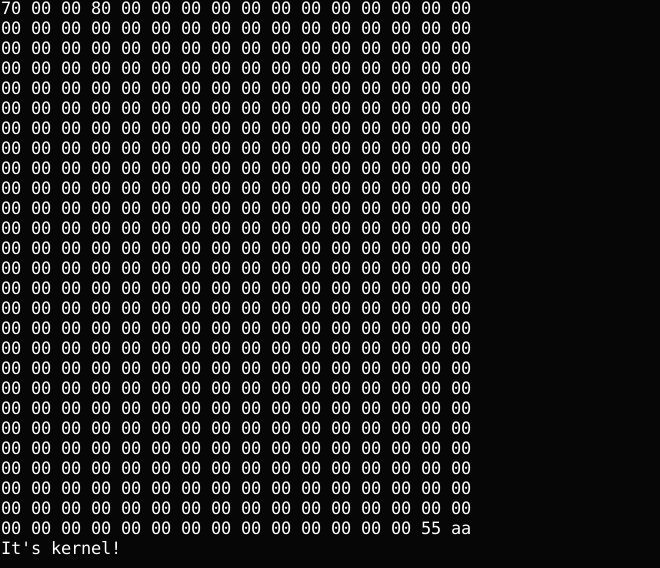
\includegraphics[height = 9cm, width = 
	13cm]{fig/4.2.png}\caption{串口输出\emph{It's kernel!}}
\end{figure}

\section*{四、关键函数功能}
1.$read\_exec\_file()$函数

代码:
\begin{lstlisting}[language=c]
Elf32_Phdr * read_exec_file(FILE **execfile, Elf32_Ehdr **ehdr)
{
  *ehdr = (Elf32_Ehdr *) malloc (512 * sizeof(uint8_t));
  fread( *ehdr, 512, 1, *execfile );
  Elf32_Phdr *phdr;
  phdr = (Elf32_Phdr *) malloc ((512 - (*ehdr)->e_phoff) * sizeof(uint8_t));
  fseek(*execfile, (*ehdr)->e_phoff, SEEK_SET);
  fread (phdr, 512 - (*ehdr)->e_phoff, 1, *execfile );
  return phdr;
}
\end{lstlisting}
函数参数为文件指针的地址以及一个$Elf32\_Ehdr$指针的地址,然后,首先给$*ehdr$分配内存,之后,读取$ELF$
文件,然后根据文件头表信息读取程序头表,再将程序头表的地址返回。\\

2.$write\_boot()$函数

代码:
\begin{lstlisting}[language=c]
void write_boot(FILE **imagefile, FILE *boot_file, Elf32_Ehdr *boot_header,
Elf32_Phdr *boot_phdr, int *count)
{
  int i;
  for ( i = 0; i < boot_header->e_phnum; i++ ) {
    if( boot_phdr[i].p_type == PT_LOAD ){//need write to image
      *count += boot_phdr[i].p_filesz;
      int test = fseek(boot_file, boot_phdr[i].p_offset, SEEK_SET);//seek to 
      the beginning of the section
      assert(!test);
      //read to buf and write to image
      uint8_t buf[boot_phdr[i].p_filesz];
      fread(buf, boot_phdr[i].p_filesz, 1, boot_file);
      fwrite(buf, boot_phdr[i].p_filesz, 1, *imagefile);
      }
  }
//write zero to the left bytes
  uint8_t zero[512 - *count - 2 ];
  for ( i = 0; i < 512 - *count -2 ; i++ ) {
    zero[i] = 0;
  }
//write 0x55 and 0xaa to the last two bytes of the first sector.
  uint8_t end[2] = {85,170};
  fwrite(zero, 512 - *count - 2, 1, *imagefile);
  fwrite(end, 2, 1, *imagefile);
}
\end{lstlisting}
写镜像的基本过程已经在前面说过,需要注意的地方是:$bootblock$占一个扇区,而可执行程序段不足$512$个字节,
因此不足的地方需要补$0$。另外,扇区的最后两个字节需要写入$0x55$和$0xaa$,标识扇区的结束。
$write\_kernel()$函数和该函数基本一样,唯一不同的地方是最后算出总的字节数目,然后模$512$,
剩下不足$512$
的地方全部补$0$。\\

3.$count\_kernel\_sectors()$函数

代码:
\begin{lstlisting}[language=c]
int count_kernel_sectors(Elf32_Ehdr *kernel_header, Elf32_Phdr *kernel_phdr){
  int i, count = 0;
  for ( i = 0; i < kernel_header->e_phnum; i++ ) {
  if ( kernel_phdr[i].p_type == PT_LOAD )
    count += kernel_phdr[i].p_filesz;
  }
  return (count + 511) >> 9;
}
\end{lstlisting}
首先计算出可加载程序段的字节数,然后加上$511$,再除以$512$即得扇区数,而除以$512$也就是右移$9$位。
由于移位效率更高,因此用移位来代替除法。\\

4.$record\_kernel\_secrots()$函数

代码:
\begin{lstlisting}[language=c]
void record_kernel_sectors(FILE **image_file, int num_sec){
  int test = fseek(*image_file, 0x40, SEEK_SET);//seek to the second inst of 
  bootblock
  assert( !test );
  int inst_li = 0x24060000 + 0x200 * num_sec; //LI $6, 0x200 * num_sec
  fwrite(&inst_li, 4, 1, *image_file );//modify the image file
}
\end{lstlisting}
通过直接修改$bootblock$中对应的$nop$指令来实现传参。\\

5.$extended\_opt()$函数

部分代码:
\begin{lstlisting}[language=c]
  #include<sys/stat.h>
  struct stat buf_boot, buf_kernel;
  stat("bootblock", &buf_boot);
  stat("kernel", &buf_kernel);
  printf("length_of_bootblock=%d\n", (int)buf_boot.st_size);
  printf( "length_of_kernel=%d\n", (int)buf_kernel.st_size );
\end{lstlisting}
该函数需要打印的相关信息基本都可以通过文件头表和程序头表获取,只有文件的长度需要调用$stat()$函数来获取。

\section*{五、疑问}
龙芯不同版本的$gcc$编译器不兼容?

前两天,我在自己的$Linux$系统上配置交叉编译环境,没有使用$3.6$版本的$mipsel-linux-gcc$,而是使用$4.3$版本的$mipsel-linux-gcc$,结果原本正确的代码上板却不能运行。于是,我又从虚拟机中把$3.6$
版本的$gcc$拷到主机中来编译,能够正常工作。然后我对比了一下两个版本的$gcc$编译出来的$bootblock$和$kernel$,发现$4.3$版本的优化了更多指令,指令数更少。不明白为什么两个版本之间会有这么大的区别,以至于不能
工作。

\section*{六、参考文献}

无。
\end{document}

